\section{Introduction}\label{sec:intro}

\parbf{Tree comparison.}
We will denote by $|a-b|_X$ the distance between points $a$ and $b$ in the metric space $X$.

Let $(a_1,\dots a_n)$ be a point array in a metric space $X$ and $T$ be a 
tree with the vertexes labeled by $\{a_1,\dots,a_n\}$.
We say that $(a_1,\dots a_n)$  satisfies the \emph{$T$-tree comparison} if there is a point array $(\~a_1,\dots, \~a_n)$ in the Hilbert space $\HH$ such that 
\[|\~a_i-\~a_j|_\HH\ge|a_i-a_j|_X\]
for any $i$ and $j$ and the equality holds if $a_i$ and $a_j$ are adjacent in $T$.

We say that a metric space $X$ satisfies the \emph{$T$-tree comparison} if 
every $n$-points arrays in $X$ satisfies the $T$-tree comparison.

\hide
\begin{wrapfigure}{r}{27 mm}
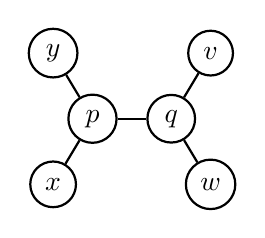
\begin{tikzpicture}[scale=1,
  thick,main node/.style={circle,draw,font=\sffamily\bfseries,minimum size=3mm}]
  \node[main node] (1) at (-1/2,-5/6) {$x$};
  \node[main node] (2) at (0,0){$p$};
  \node[main node] (3) at (-1/2,5/6){$y$};
  \node[main node] (4) at (3/2,5/6) {$v$};
  \node[main node] (5) at (1,0) {$q$};
  \node[main node] (6) at (3/2,-5/6) {$w$};

  \path[every node/.style={font=\sffamily\small}]
   (1) edge node[above]{}(2)
   (2) edge node[above]{}(3)
   (2) edge node[above]{}(5)
   (4) edge node[above]{}(5)
   (5) edge node[above]{}(6);
\end{tikzpicture}
\end{wrapfigure}
\unhide

\parbf{Encoding of trees.}
To encode the labeled tree on the diagram, we will use notation $p/xy(q/vw)$.
It means that we choose $p$ as the root; 
$p$ has two children leafs to $x$, $y$ and one child $q$ with two children leafs $v$ and $w$.
Taking another root for the same tree, we get different encodings, for eaxample $q/vw(p/xy)$ or $x/(p/y(q/vw))$.

If we do not need the labeling of vertexes,
it is sufficient to write the number of leafs in the brackets;
this way we can write 2(2) instead of $p/xy(q/vw)$ since the root ($p$) has two leafs ($x$ and $y$) and yet another child ($q$) has two leafs ($v$ and $w$).  
The same tree can be written as (1(2)) meaning that the root $x$ has no leafs, $p$ has one leaf $y$ and one child $q$ with two leafs $v$ and $w$.
Every vertex which is not the root and not a leaf corresponds to a pair of bracketsin this notation.


Using the described notation, we could say that a metric space \emph{satisfies the 2(2)-tree comparison},  meaning that it satisfies the tree comparison on the diagram.
We could also say \emph{``applying the $p/xy(q/vw)$-tree comparison we get...''} meaning that we apply the comparison for these 6 points and the tree on the diagram.

A vertex of a tree is called \emph{pole}
that is they have one vertex (\emph{pole}) adjacent to all other vertexes.

\hide
\begin{wrapfigure}{r}{20 mm}
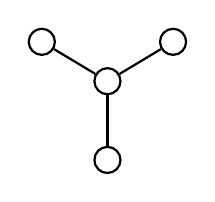
\begin{tikzpicture}[scale=1,
  thick,main node/.style={circle,draw,font=\sffamily\bfseries,minimum size=3mm}]

  \node[main node] (1) at (5/6,1) {};
  \node[main node] (2) at (0,3/2){};
  \node[main node] (3) at (10/6,3/2){};
  \node[main node] (4) at (5/6,0) {};

  \path[every node/.style={font=\sffamily\small}]
   (1) edge node[above]{}(2)
   (1) edge node[above]{}(3)
   (1) edge node[above]{}(4);
\end{tikzpicture}
\end{wrapfigure}
\unhide

\parbf{Monopolar comparisons.}
We define \emph{Alexandrov space} as complete length space with curvature bounded below in the sense of Alexandrov;
the latter is equivalent to the 3-tree comparison for the tripod-tree on the diagram. 

Using the introduced notation, Theorem 4.1. in \cite{AKP} can be restated the following way: \emph{If length-metric space satisfies $3$-tree comparison, then it also satisfies $n$-tree comparison for every positive integer~$n$.}

In this example the trees are \emph{monopolar};
that is, they have one pole.

\parbf{Dipolar comparison.} 
A tree will be called \emph{dipoar} if it has exactly two poles;
that is, two vertexes of degree at least two.

Equivalently, dipolar trees could be defined as the trees with diameter 3
or as the trees which admit an encoding $m(n)$ for positive integers $m$ and $n$; 
in this tree $m$ vertexes are adjacent to the first pole which is the root
and $n$ vertexes are adjacent to the second pole and the two poles are adjacent.

In Section~\ref{6-dipole} we will show that the comparison for the any Alexandrov space with nonnegative curvature satisfies the comparisons for the trees 2(2) and 3(1) --- the first two trees an the following diagram.

\hide
\begin{center}

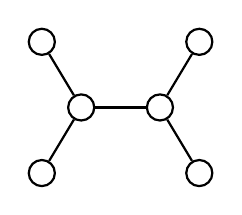
\begin{tikzpicture}[scale=1,
  thick,main node/.style={circle,draw,font=\sffamily\bfseries,minimum size=3mm}]

  \node[main node] (1) at (0,0) {};
  \node[main node] (2) at (1/2,5/6){};
  \node[main node] (3) at (0,10/6){};
  \node[main node] (4) at (2,0) {};
  \node[main node] (5) at (3/2,5/6) {};
  \node[main node] (6) at (2,10/6) {};

  \path[every node/.style={font=\sffamily\small}]
   (1) edge node[above]{}(2)
   (2) edge node[above]{}(3)
   (2) edge node[above]{}(5)
   (4) edge node[above]{}(5)
   (5) edge node[above]{}(6);
\end{tikzpicture}
\hskip10mm
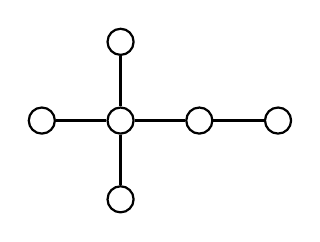
\begin{tikzpicture}[scale=1,
  thick,main node/.style={circle,draw,font=\sffamily\bfseries,minimum size=3mm}]

  \node[main node] (1) at (1,2) {};
  \node[main node] (2) at (1,0){};
  \node[main node] (3) at (1,1){};
  \node[main node] (4) at (0,1) {};
  \node[main node] (5) at (3,1) {};
  \node[main node] (6) at (2,1) {};

  \path[every node/.style={font=\sffamily\small}]
   (1) edge node[above]{}(3)
   (2) edge node[above]{}(3)
   (3) edge node[above]{}(6)
   (4) edge node[above]{}(3)
   (5) edge node[above]{}(6);
\end{tikzpicture}
\end{center}
\unhide


\parbf{CTP, MTW and CTIL.}
In Section~\ref{7-dipole}, we will show that the comparison for the tree 4(1) (see the diagram below) implies
the curvature condition introduced by Ma--Trudinger--Wang (briefly MTW condition) and convexity of tangent injectivity loci (briefly CTIL condition).

\hide
\begin{center}
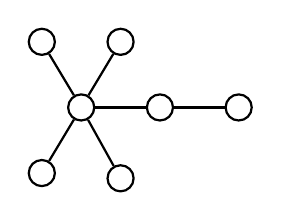
\begin{tikzpicture}[scale=1,
  thick,main node/.style={circle,draw,font=\sffamily\bfseries,minimum size=3mm}]

  \node[main node] (0) at (3/2,11/6){};
   \node[main node] (1) at (1/2,1/6){};
  \node[main node] (2) at (3/2,.1){};
  \node[main node] (3) at (1,1){};
  \node[main node] (4) at (1/2,11/6){};
  \node[main node] (5) at (3,1){};
  \node[main node] (6) at (2,1){};

  \path[every node/.style={font=\sffamily\small}]
     (0) edge node[above]{}(3)
   (1) edge node[above]{}(3)
   (2) edge node[above]{}(3)
   (3) edge node[above]{}(6)
   (4) edge node[above]{}(3)
   (5) edge node[above]{}(6);
\end{tikzpicture}

\end{center}
\unhide

These two conditions appear in the study of continuity of optimal transport between regular measures with positive continuous density functions.
The continuity implies both MTW and CTIL conditions and slightly stronger version of these two conditions imply the continuity;
see \cite{FRV-Nec+Suf}, \cite{MTW+CTIL} and the references there in.

%MORE???

Note that dipolar comparison provides a uniform way to treat combined CTIL+MTW condition;
this partially answers the question of Cédric Villani in ???.

Note that 4(1)-tree comparison (as well as any $T$-tree comparison) is stable under passing to the limit.
Namely, if a sequence of metric spaces $X_n$ satisfies 4(1)-comparison and converges in the sense of Gromov--Hausdorff to the space  then its limit $X_\infty$ also satisfies 4(1)-comparison.

We expect that for Riemannian manifolds, the 4(1)-tree comparison is equivalent to CTP and to MTW+CTIL (see question ???).
If this is indeed the case then from above it will follow that the properties CTP and MTW+CTIL are stable as well.

\parbf{All tree comparisons.}
In Section~\ref{sec:all-tree} we show that if the space satisfies all tree comparisons then it is a target space of submetry from a subset in Hilbert space.

We also show that all bi-quotients of compact Lie groups with bi-invariant metrics satisfy all tree comparison.

